\scanpage{47}
\mspage{- 22 -}
% archive sheet number: 46

COROLLAIRE.- \uline{Soit} $\handwritten{u}(z_1,..,z_p)$ \uline{une fonction holomorphe dans une partie ouverte} $A$ \uline{de} $K^p$, \uline{à valeurs dans} $K^p$. \uline{Pour tout point} $\handwritten{a}=(a_1,\ldots,a_p)$ \uline{de} $A$ \uline{tel que la différentielle} $\handwritten{\unsure{d.u(a)|du(a)}}$ \uline{soit inversible il existe un voisinage ouvert} $U$ \uline{de} $\handwritten{a}$ \uline{tel que la restriction de} $\handwritten{u}$ \uline{à} $U$ \uline{soit un homéomorphisme de} $U$ \uline{sur un voisinage ouvert} $V$ \uline{de} $\handwritten{u(a)}$, \uline{et que l'homéomorphisme réciproque soit holomorphe dans} $V$.

% The brown marginal outline is visible; whether it is ink or adhering material is uncertain.
\margin{\figure{\handwritten{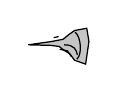
\begin{tikzpicture}[x=0.7cm,y=0.7cm,line width=0.45pt]
\filldraw[fill=gray!45] (0.68,0.30) -- (0.90,0.34) -- (0.94,0.10) -- (0.88,-0.31) -- (0.68,-0.24) -- (0.59,-0.12) -- (0.49,-0.06) -- (0.40,0.01) -- (0.25,0.03) -- (-0.16,0.04) -- (0.26,0.10) -- (0.47,0.14) -- (0.58,0.23) -- cycle;
\draw (0.69,0.27) .. controls (0.80,0.18) and (0.82,-0.14) .. (0.72,-0.22);
\draw (0.49,0.04) .. controls (0.68,0.04) and (0.71,-0.05) .. (0.73,-0.14);
\draw (0.41,-0.04) -- (0.55,-0.07) -- (0.62,-0.17);
\draw (0.30,0.17) -- (0.39,0.19);
\end{tikzpicture}}}}
Lorsque $K=\handwritten{\unsure{R|\mathbb{R}}}$ et que $A$ est un intervalle ouvert dans $\handwritten{R}$, le fait que $u'(x)\handwritten{\ne}0$ dans $A$ entraîne que $u$ est un homéomorphisme de $A$ \uline{tout entier} sur $u(A)$ puisque $u$ est monotone dans $A$ (\uline{Fonct.var.réelle}, chap.I,\handwritten{\S}\,2 et \uline{Top.gén.} chap.IV,\handwritten{\S}\,2). Mais lorsque $K=\handwritten{\mathbb{C}}$, $u'(x)$ peut être $\handwritten{\ne}0$ en tout point d'un domaine $A\handwritten{\subset C}$ sans que $u$ soit un homéomorphisme de $A$ sur $u(A)$. Par exemple, si $u(x)=x^n$, on a $u'(x)\handwritten{\ne}0$ pour $x\handwritten{\ne}0$, mais si $A$ est le disque $\handwritten{|}x-1\handwritten{|<\frac{1}{2}}$, $u$ n'est pas un homéomorphisme de $A$ sur $u(A)$ dès que $n$ est assez grand, car il existe des points $x\handwritten{\ne}1$ dans $A$ tels que $x^n=1$.

Il faudrait faire ici également le théorème de \uline{dépendance} des fonctions holomorphes à jacobien identiquement nul.

\handwritten{\uline{3}}. \uline{Intégration des équations différentielles}.

THEOREME 2.- \uline{Soit} $K$ \uline{un corps valué complet de caractéristique} $0$. \uline{Soient} $f_i(x;y_1,..,y_p;z_1,..,z_q)$ $(1\handwritten{\leq}i\handwritten{\leq}p)$ $p$ \uline{fonctions holomorphes scalaires définies dans une partie ouverte} $A$ \uline{de} $K^{p+q+1}$. \uline{Pour tout point} $(a;b_1,..,b_p;c_1,..,c_q)$ \uline{de} $A$, \uline{il existe un voisinage} $U$ \uline{de} $a$ \uline{dans} $K$, \uline{un voisinage} $V$ \uline{de} $(b_1,..,b_p)$ \uline{et un voisinage} $W$ \uline{de} $(c_1,..,c_q)$ \uline{tels que} $U\handwritten{\times}V\handwritten{\times}W\handwritten{\subset}A$, \uline{et un système et un seul de} $\uline{p}$ \uline{fonctions scalaires} $u_i(x;z_1,..,z_q)$, \uline{holomorphes dans} $U\handwritten{\times}W$\handwritten{,} \uline{telles que l'image de} $U\handwritten{\times}W$ \uline{par l'application} $(x;z_1,..,z_q)\handwritten{\to}(u_i(x;z_1,\ldots,z_q))$ \uline{soit contenue dans} $V$ \uline{et qui satisfont dans} $U\handwritten{\times}W$ \uline{aux conditions}
